\documentclass[11pt,a4paper]{article}

% Packages and formatting


\usepackage{float}
\usepackage{amsmath}
\usepackage{amssymb}
\usepackage[parfill]{parskip}
\usepackage{graphicx}
\usepackage[numbers]{natbib}
\usepackage[hidelinks]{hyperref}
\usepackage[margin=1in]{geometry}
\usepackage{booktabs}
\usepackage{tabularx}
\usepackage{tikz}

\usepackage{listings}
\usepackage{xcolor}


\usetikzlibrary{positioning,arrows.meta}
\graphicspath{{../reports/figures/}}

\lstdefinelanguage{json}{
    morestring=[b]",
    stringstyle=\color{blue!55!black},
    morekeywords={true,false,null},
    keywordstyle=\color{purple!65!black},
    sensitive=false,
    showstringspaces=false
}

\lstdefinestyle{jsonstyle}{
    language=json,
    basicstyle=\ttfamily\scriptsize,
    breaklines=true,
    breakatwhitespace=false,
    columns=fullflexible,
    keepspaces=true,
    frame=single,
    rulecolor=\color{black!20},
    backgroundcolor=\color{gray!3},
    numbers=left,
    numberstyle=\tiny\color{gray},
    numbersep=7pt,
    xleftmargin=12pt,
    framexleftmargin=8pt,
    tabsize=2,
    showstringspaces=false,
    captionpos=b
}

\title{\textbf{Beyond Retrieval: Scope-Aware Memory Application in AI Agents}}

\author{
\begin{tabular}{cc}
    Isaac Chin Wei En & Edward Chew Kian Boon \\
    \small A0248885H & \small A0271710N \\[1em]
    Ng Cheng Kiat Nicholas & Jagan Mohan Shailesh \\
    \small A0271938R & \small A0272542H
\end{tabular}
}

\date{}


\begin{document}
\maketitle

\begin{abstract}
Long-term memory enables language-model agents to retain user
preferences across interactions, but retrieving a relevant memory
does not guarantee that the agent applies it in the correct context.
We investigate scope-aware memory application by augmenting Mem0
and Supermemory with write-time and read-time scope tagging.
We construct a benchmark of 40 episodes in 20 paired scenarios,
covering five types of conflicting instructions, and evaluate eight
conditions across 320 runs. The expected memory was retrieved in
43 of 51 incorrect responses across the six memory-system conditions,
demonstrating a substantial retrieval--application gap. Read-time
tagging with Supermemory achieves the highest observed adherence
(92.5\%), compared with 85\% for its baseline, although this
difference is not statistically significant ($p=0.25$). Write-time
tagging scored lower than the baseline for both systems; for Mem0 it
also scored lower than read-time tagging (60\% vs 80\%, $p=0.039$),
which we trace to Mem0 re-extracting the pre-tagged instructions. These
findings suggest that explicit scope information may support memory
application, but its effectiveness depends on how it is integrated
and used.
\end{abstract}

\section{Introduction}

\subsection{Motivation and Research Problem}

Memory-augmented language-model agents retain user instructions
across conversations, allowing responses to reflect previously
expressed preferences. However, preferences are not always
universally applicable. A user may generally prefer Polars for
large datasets while requiring pandas for a particular group
project. Both memories remain valid, but the appropriate action
depends on the current context.

Existing memory systems primarily address the storage and
retrieval of relevant information. Yet even when conflicting
instructions are successfully retrieved, an agent must determine
which instruction applies, whether an exception overrides a
standing preference, and whether a temporary instruction should
continue to influence subsequent tasks.

We investigate this distinction between \emph{memory retrieval}
and \emph{memory application}: does an agent correctly use a
retrieved instruction within its intended scope, and can explicit
scope information improve its decisions?

\subsection{Research Objectives and Contributions}

We investigate two questions: (1) whether agents make incorrect
decisions despite retrieving the expected memory, and (2) whether
scope-aware interventions improve contextual adherence while
preserving unrelated preferences.

Our contributions are:
\begin{enumerate}
    \item A lightweight scope-tagging layer supporting standing,
    project-specific, and single-task instructions, integrated
    with Mem0 and Supermemory at write time or read time.
    \item A synthetic benchmark of 20 paired scenarios (40
    episodes) covering five memory-conflict categories.
    \item An evaluation of eight conditions across 320 runs,
    separating retrieval success, memory application, scope
    errors, tagging accuracy, and unrelated-memory retention.
\end{enumerate}

\section{Related Work}

\subsection{Long-Term Memory in LLM Agents}

Mem0~\cite{chhikara2025mem0} provides persistent agent memory
through extraction, storage, updating, and retrieval of
information from interactions. Supermemory
\cite{supermemoryresearch} offers a hosted memory service with
ingestion and semantic search. Both aim to make relevant prior
information available to agents without repeatedly supplying
complete conversation histories.

Our work uses these systems as memory backends rather than
proposing another storage or retrieval mechanism. We evaluate
whether their retrieved information supports contextually
appropriate decisions.

Existing long-term memory benchmarks mainly score recall.
LongMemEval~\cite{wu2025longmemeval} and
LoCoMo~\cite{maharana2024locomo} test whether an assistant
answers questions about earlier conversations (LoCoMo also
covers event summarisation and dialogue generation), and
ConvoMem~\cite{pakhomov2025convomem} compares RAG-based memory
systems, including Mem0, with placing the whole history in
context. Our benchmark differs
in what it scores: not whether a fact can be recalled, but
whether the retrieved instruction is applied inside its scope
and left unapplied outside it.

\subsection{Memory Retrieval and Contextual Applicability}

Retrieval relevance and contextual applicability are distinct.
A memory may be relevant to the current topic but inapplicable
to the current project, task, or condition. Conversely, a
retrieved exception may need to override a broader preference
without permanently replacing it.

We focus on this downstream decision problem by representing
scope explicitly and evaluating both correct application and
incorrect application beyond a memory's intended context.

\section{Methodology}
\label{sec:methodology}

\subsection{Scope Representation and Conflict Resolution}
\label{sec:scope-representation}

Each instruction is represented by three fields:
\emph{scope}, \emph{key}, and \emph{condition}.
The scope determines applicability, the optional key identifies
a project or task, and the optional condition specifies an
additional constraint.

\begin{table}[htbp]
\centering
\small
\caption{Scope representation.}
\label{tab:scopes}
\begin{tabularx}{\linewidth}{lXl}
\toprule
Scope & Applicability & Example \\
\midrule
Standing & General preference across tasks &
Use Polars \\
Project & Restricted to a named project &
Marlin: pandas \\
Single-task & Restricted to one task &
This export: CSV \\
\bottomrule
\end{tabularx}
\end{table}

The reference decision policy first excludes memories whose
project, task, or condition does not match the current request.
Among applicable memories concerning the same decision, scope
precedence is
\[
\text{single-task} \succ \text{project}
\succ \text{standing}.
\]
Within one scope, an applicable conditional instruction takes
precedence over an unconditional instruction; recency resolves
remaining conflicts at equal specificity. Unrelated instructions
do not compete, and the benchmark excludes unresolved ties.

These rules define the reference actions and are communicated
to the agent. The scope layer does not deterministically
select the winning memory.

\subsection{Scope-Tagging Architecture}
\label{sec:architecture}

We augment Mem0~\cite{chhikara2025mem0} and
Supermemory~\cite{supermemoryresearch} with an LLM-based
scope tagger. Figure~\ref{fig:architecture} compares the
two integration strategies.


\begin{figure}[htbp]
\centering
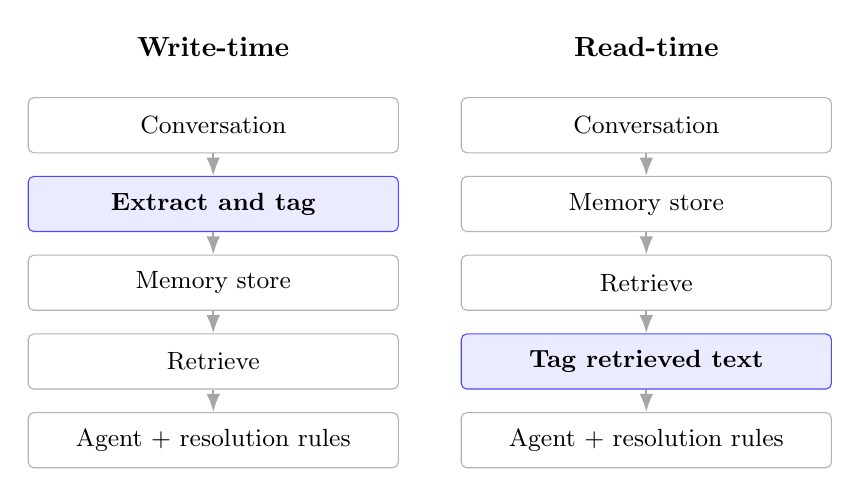
\begin{tikzpicture}[
    >=Latex,
    node distance=0.55cm,
    box/.style={
        draw=gray!60,
        rounded corners=2pt,
        minimum width=4.7cm,
        minimum height=0.7cm,
        align=center,
        font=\small
    },
    tag/.style={
        box,
        draw=blue!70,
        fill=blue!8,
        font=\small\bfseries
    },
    arrow/.style={->,thick,gray!70}
]

% Column headings
\node[font=\bfseries] at (0,0) {Write-time};
\node[font=\bfseries] at (5.5,0) {Read-time};

% Write-time pipeline
\node[box] (w1) at (0,-1) {Conversation};
\node[tag] (w2) at (0,-2) {Extract and tag};
\node[box] (w3) at (0,-3) {Memory store};
\node[box] (w4) at (0,-4) {Retrieve};
\node[box] (w5) at (0,-5) {Agent + resolution rules};

% Read-time pipeline
\node[box] (r1) at (5.5,-1) {Conversation};
\node[box] (r2) at (5.5,-2) {Memory store};
\node[box] (r3) at (5.5,-3) {Retrieve};
\node[tag] (r4) at (5.5,-4) {Tag retrieved text};
\node[box] (r5) at (5.5,-5) {Agent + resolution rules};


% Write-time arrows
\draw[arrow] (w1.south) -- (w2.north);
\draw[arrow] (w2.south) -- (w3.north);
\draw[arrow] (w3.south) -- (w4.north);
\draw[arrow] (w4.south) -- (w5.north);

% Read-time arrows
\draw[arrow] (r1.south) -- (r2.north);
\draw[arrow] (r2.south) -- (r3.north);
\draw[arrow] (r3.south) -- (r4.north);
\draw[arrow] (r4.south) -- (r5.north);


\end{tikzpicture}
\caption{Scope-tagging integration strategies.
Write-time tagging occurs before storage, whereas
read-time tagging occurs after retrieval.}
\label{fig:architecture}
\end{figure}


Write-time tagging extracts individual instructions from the
full conversation and stores them with scope metadata. It
can preserve scope cues early but may discard surrounding
conversational context. Read-time tagging operates on the
memory system's retrieved text, preserving native storage
behaviour but relying on that text to retain sufficient
contextual information.

Both strategies supply tagged memories and conflict-resolution
rules to the agent. Structured task identifiers are withheld
from the taggers, so task continuity must be inferred from
natural-language context.

The two memory systems return different units. Mem0 extracts and
rewrites short notes. Supermemory's search returns raw
session passages (retrieved items begin ``User: \ldots\
Assistant: \ldots''), so its baseline prompt is close to the full
transcript in size (444 vs 465 tokens per episode on average).
A read-time tag on a Supermemory result therefore labels a whole
passage with one scope, even when the passage holds several
instructions.

In the write-time variants each tagged instruction is stored with
its tag as metadata through the system's normal write call. For
Mem0 that call runs its default extraction (\texttt{infer=True}), so
the pre-extracted instruction is rewritten again before storage.

\subsection{Benchmark Construction}
\label{sec:benchmark}

\subsubsection{Episode Structure and Mirrored-Pair Design}

We construct 20 paired scenarios containing 40 episodes.
Each pair includes two or three earlier conversation sessions,
reference memories, and two probes sharing the same history.
Probe A tests an applicable scoped instruction; Probe B
changes the project, task, or condition so that the instruction
no longer applies. Each episode consists of one probe and
its shared history, with an expected action for evaluation.

Each pair also includes an unrelated standing preference and
a retention check. Pair accuracy requires both probes to be
correct, discouraging fixed choices that ignore context.

For example, pair \texttt{po-01} combines a standing preference
for Polars on datasets exceeding one million rows with a
project-specific instruction to use pandas for Project Marlin.



\begin{figure}[htbp]
    \centering
    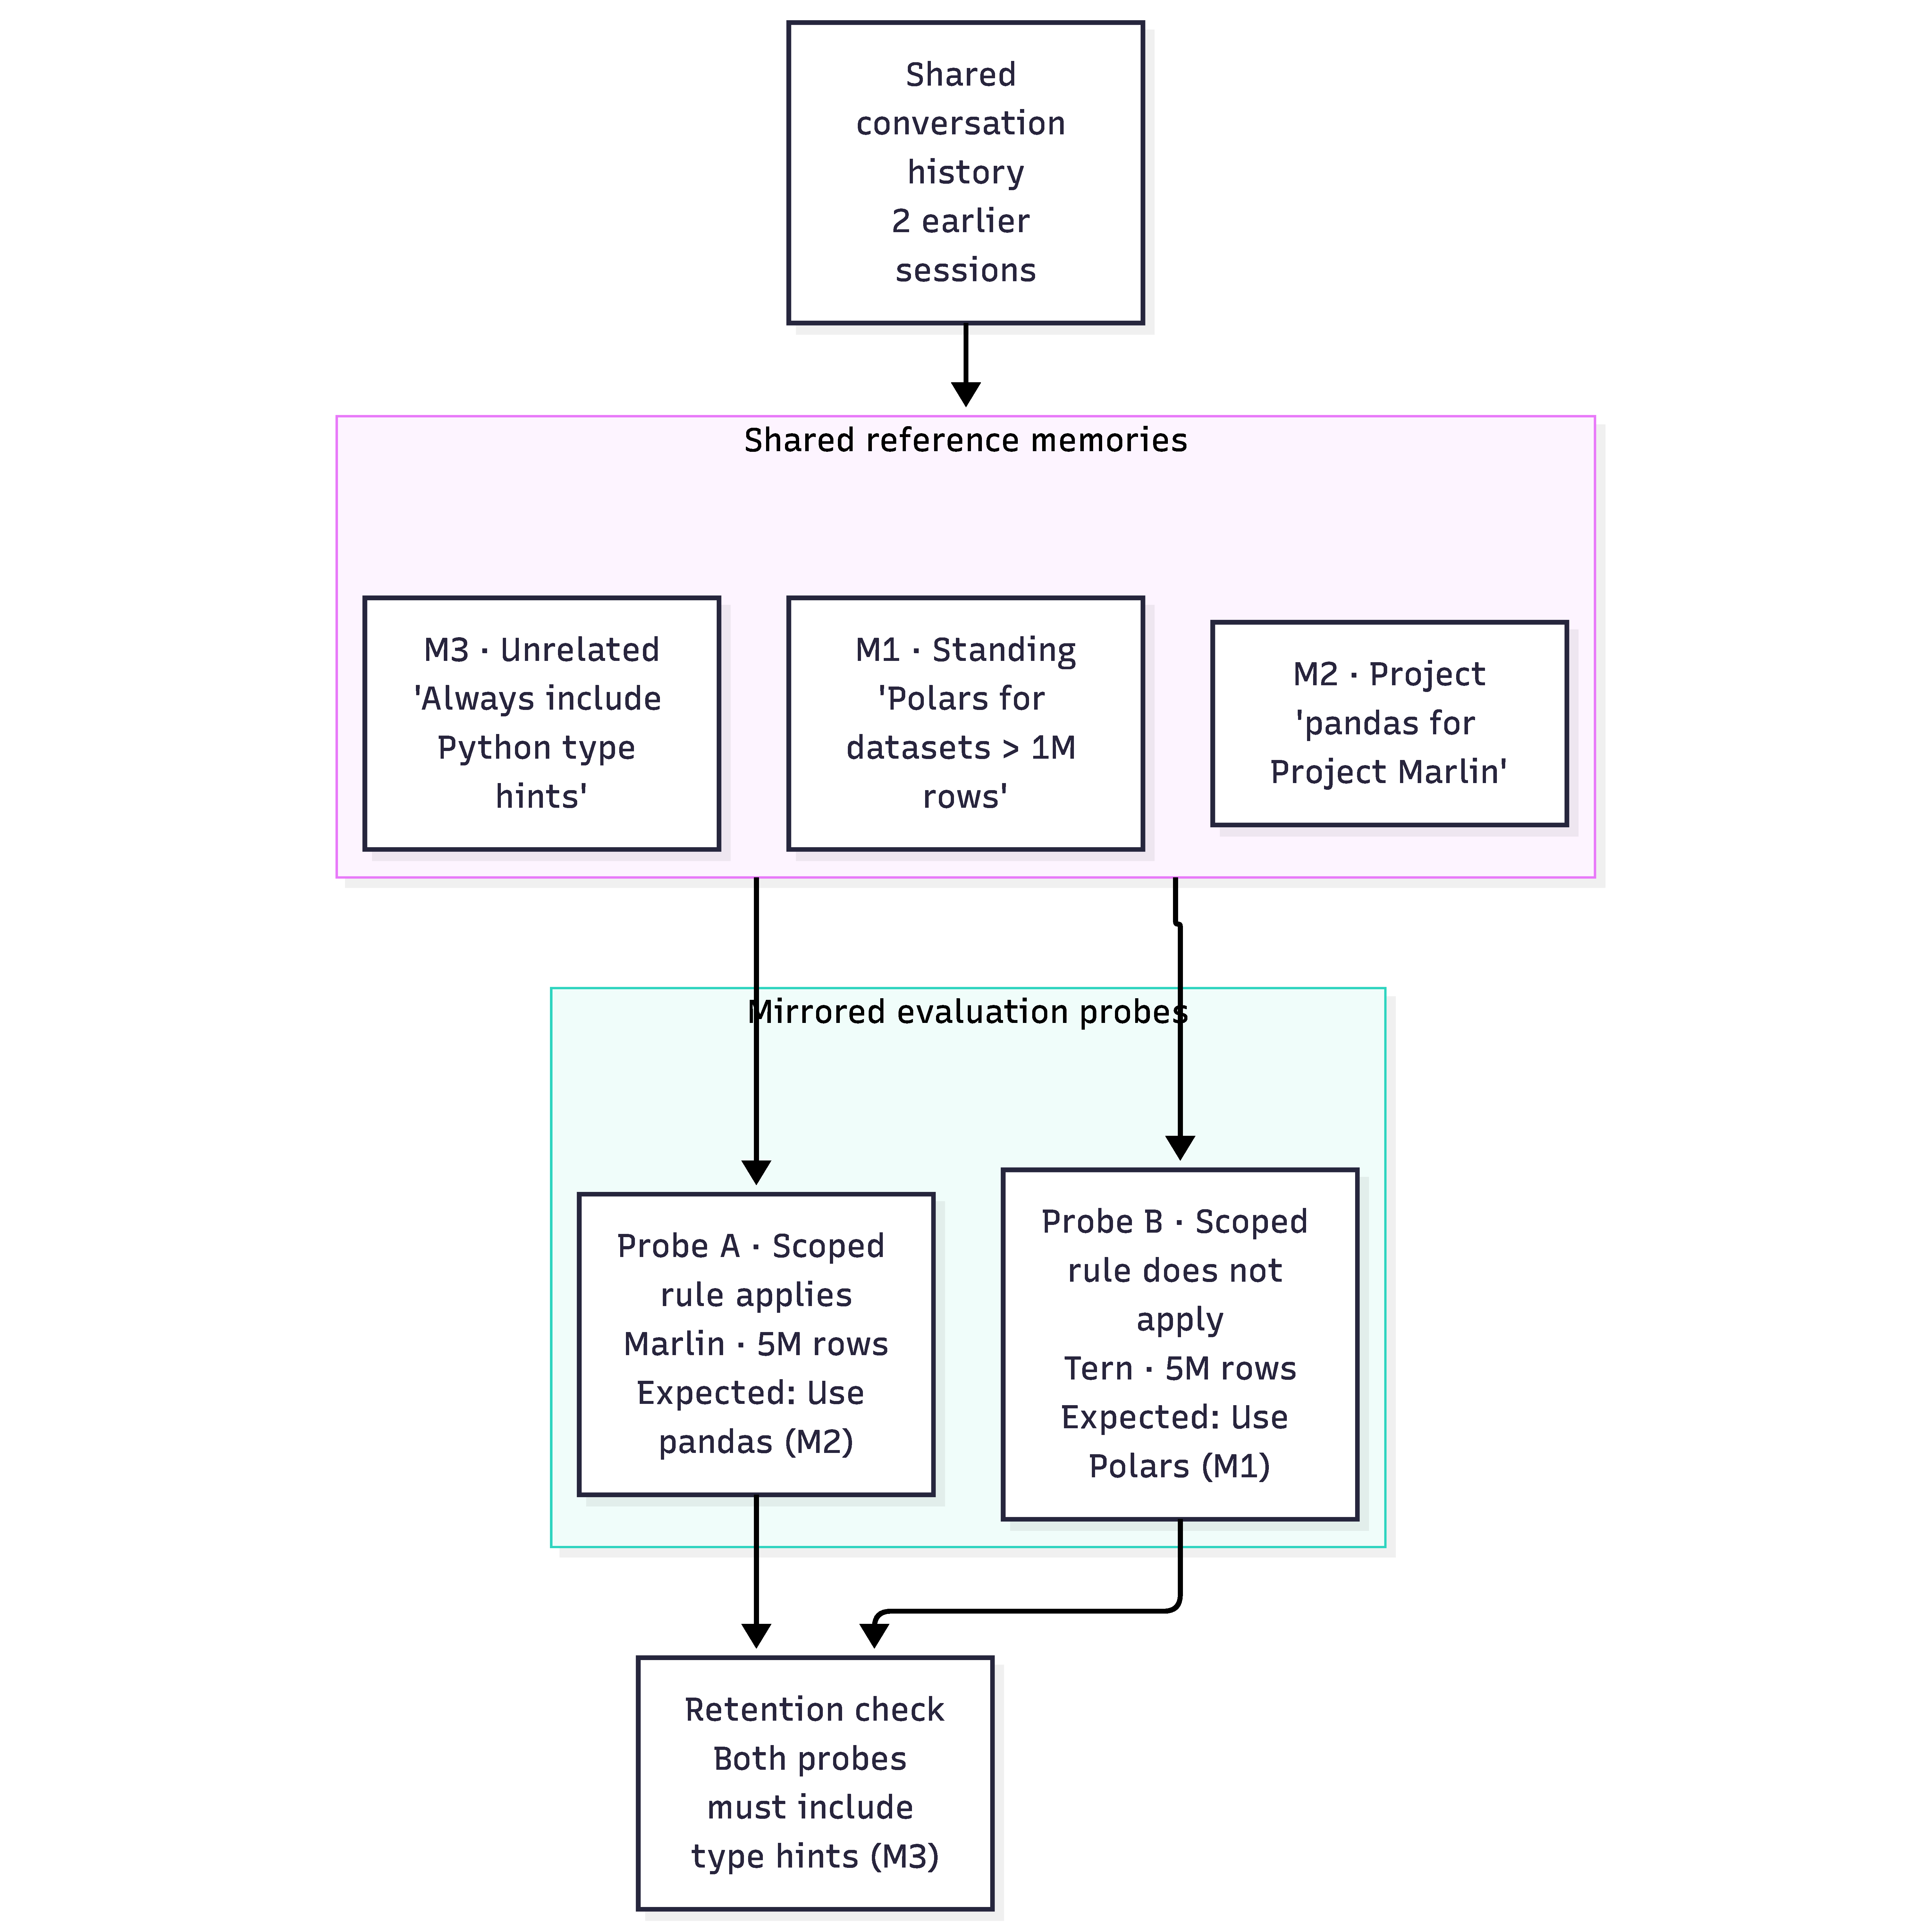
\includegraphics[width=0.85\linewidth]{mirrored_pair_design.pdf}
    \caption{Mirrored-pair benchmark design illustrated
    using pair \texttt{po-01}. Both probes share the
    same conversation history and reference memories
    but differ in whether the project-specific instruction
    applies. An unrelated standing preference is
    evaluated independently in both probes.}
    \label{fig:mirrored-pair}
\end{figure}





\subsubsection{Conflict Categories and Dataset Generation}

The benchmark covers five conflict categories, with four
pairs per category:

\begin{table}[htbp]
\centering
\small
\caption{Benchmark composition.}
\label{tab:benchmark}
\begin{tabular}{lrr}
\toprule
Conflict category & Pairs & Episodes \\
\midrule
Project override & 4 & 8 \\
Single-task override & 4 & 8 \\
Conditional scope & 4 & 8 \\
Same-scope supersession & 4 & 8 \\
Same-scope specificity & 4 & 8 \\
\midrule
Total & 20 & 40 \\
\bottomrule
\end{tabular}
\end{table}

The categories test project exceptions, temporary task
exceptions, conditional applicability, replacement of older
instructions within one scope, and precedence of more
specific instructions within one scope.

The 20 pairs contain 66 distinct reference memories,
including competing and unrelated instructions.
Nineteen pairs were initially drafted with AI assistance
and subsequently reviewed and revised. The suite varies
domains, wording, chronology, and instruction positions;
some standing preferences deliberately appear after
narrower instructions.

\subsubsection{Dataset Validation and Gold Labels}

Automated checks validate the JSON schema, verbatim
memory quotations, paired-probe similarity, expected
decisions, and diversity. Only session and probe text
reach the systems; structured gold labels and expected
actions are withheld. A leakage test checks this
separation.

The 66 memories were reviewed against the drafted labels. The
reviewed labels matched the drafts on scope and
key for all 66 memories and differed on four condition
expressions (94\% condition agreement); the original reference
expressions were retained. The two committed annotation files are
identical, so we report no inter-annotator agreement.
% TODO(team): confirm who labelled and whether two people labelled independently.

\subsection{Experimental Conditions and Baselines}
\label{sec:conditions}

We evaluate eight conditions: no memory, full transcript,
Mem0, Supermemory, and write-time/read-time scope-tagged
variants of each memory system.

\begin{table}[htbp]
\centering
\small
\caption{Experimental conditions.}
\label{tab:conditions}
\begin{tabularx}{\linewidth}{lX}
\toprule
Condition & Memory supplied to agent \\
\midrule
No memory & Current probe only \\
Full transcript & All earlier sessions \\
Mem0 & Native retrieved memories \\
Supermemory & Native retrieved search results \\
Mem0 + write & Pre-extracted, tagged memories \\
Mem0 + read & Retrieved memories tagged afterward \\
Supermemory + write & Pre-extracted, tagged memories \\
Supermemory + read & Retrieved results tagged afterward \\
\bottomrule
\end{tabularx}
\end{table}

Each condition evaluates all 40 episodes, yielding
320 runs. The scope-layer conditions introduce tags,
resolution rules, and memory ordering information
together; their individual effects cannot be isolated.

\section{Experimental Setup and Evaluation}
\label{sec:experimental-setup}

\subsection{Implementation and Model Configuration}

The implementation uses Python 3.11+, \texttt{uv}, and
a shared lockfile. The agent is
\path{qwen/qwen3.8-flash} through OpenRouter, with
temperature 0, seed 4213, a 1,024-token output limit,
and reasoning disabled. The agent prompt template and
sampling settings are fixed across conditions, with
retrieval limited to ten results.

Qwen was selected after an operational pilot: it
reported zero reasoning usage on 40 pilot calls,
whereas DeepSeek returned empty text on three of
eight calls when reasoning was disabled.

Both memory systems use a common interface and fresh
namespaces for each episode and condition. Mem0 uses
its default extraction and search, an
\texttt{all-MiniLM-L6-v2} embedder (384 dimensions),
Qdrant storage, and internal LLM calls through
OpenRouter. The locked environment omits Mem0's optional
spaCy and fastembed dependencies, so all Mem0 runs used
vector retrieval without BM25. Supermemory uses its hosted API
and waits for ingestion to complete before retrieval.

OpenRouter token usage and costs are recorded in an
append-only ledger. Supermemory's separately billed
processing is excluded from those costs.

\subsection{Evaluation Metrics}
\label{sec:metrics}

An LLM judge identifies the action taken in each
free-text answer. We evaluate the following metrics:

\begin{table}[htbp]
\centering
\small
\caption{Evaluation metrics.}
\label{tab:metrics}
\begin{tabularx}{\linewidth}{lX}
\toprule
Metric & Definition \\
\midrule
Adherence & Expected action selected \\
Pair accuracy & Both A and B probes correct \\
Retrieval--application gap &
Expected memory retrieved, wrong action selected \\
Retention & Unrelated standing preference followed \\
Tag accuracy & Predicted scope metadata matches reference \\
Failure stage & Earliest detected pipeline failure \\
\bottomrule
\end{tabularx}
\end{table}

Adherence is also separated into in-scope (A) and
out-of-scope (B) probes. Incorrect decisions are
classified as over-application, under-application,
supersession, or other actions.

Retrieval is checked by verbatim matching or
judge-assisted matching of rewritten notes. The
full-transcript control counts as successful retrieval
by construction; no memory counts as unsuccessful.
Retention excludes unassessable answers.

Tagging accuracy is measured on notes associated with
one reference memory. Scope is matched exactly;
project keys must contain the reference project name,
while single-task keys are excluded from scoring.
Conditions use strict (variable, operator, value)
and lenient (operator, value) matching.

Failure-stage categories are extraction, retrieval,
scope loss, tagging, and reasoning. Each incorrect
answer is assigned to the earliest detected failure.
These are diagnostic classifications, not established
causal mechanisms. Supermemory's internal extraction
cannot be inspected separately from retrieval.

\subsection{LLM-as-a-Judge and Statistical Analysis}
\label{sec:judge}

The judge uses the same Qwen model at temperature 0.
It receives the probe, response, and alphabetically
ordered candidate actions, but not the expected action.
It returns an action, \texttt{none}, or \texttt{mixed},
with supporting evidence, and separately evaluates
the retention check.

The recorded human review covers 40 action labels
and 38 assessable retention labels, with complete
agreement against the judge (Cohen's
$\kappa=1.00$)~\cite{cohen1960coefficient}.
The judge and agent share a model, so correlated
errors remain possible; LLM-judge biases are
discussed by Zheng et al.~\cite{zheng2023judging}.
Action labels can be ambiguous when an answer mixes
mechanisms. In \texttt{cs-04a} with write-time Supermemory the
answer calls \texttt{tenacity} but sets a single attempt, which
arguably implements the fail-fast instruction; the judge scored
it as the standing retry rule. We did not re-score such cases.

We report 95\% Wilson confidence intervals
\cite{wilson1927probable} and exploratory exact
McNemar tests~\cite{mcnemar1947sampling} on the
same episodes. Because the A/B probes within a
pair share history, episode-level tests do not
fully account for dependence; p-values are
interpreted cautiously.

\section{Results and Analysis}
\label{sec:results}

All 320 runs completed without execution errors.

\subsection{Overall Correction Adherence}

Figure~\ref{fig:overall-adherence} shows adherence
across the eight conditions. No memory achieves
20\% (8/40), versus 80\% (32/40) with the full
transcript. Mem0 and Supermemory achieve 77.5\%
(31/40) and 85\% (34/40).

Read-time tagging achieves 80\% with Mem0 and
92.5\% (37/40) with Supermemory, the highest
observed score. Write-time tagging scores 60\% and
77.5\%, respectively. Supermemory + read-time
resolves 17/20 complete pairs, compared with
15/20 for its baseline.

Most of these differences are within sampling noise
(Table~\ref{tab:paired}). Read-time Supermemory's
gain over its baseline (3 episodes gained, none lost,
$p=0.25$) has overlapping Wilson intervals
(80--97\% vs 71--93\%). Write-time tagging's drop
against the baselines is not significant for Mem0
($p=0.118$) or Supermemory ($p=0.549$). The one
significant adherence difference between tagging
variants is write-time against read-time Mem0
(2 episodes vs 10, $p=0.039$). Nothing is corrected
for multiple comparisons.

\begin{table}[htbp]
\centering
\small
\caption{Exact McNemar tests on the same 40 episodes
(``Only'' = episodes where only that condition was
right). Retention uses the episodes the judge could
assess.}
\label{tab:paired}
\begin{tabularx}{\linewidth}{llXrrr}
\toprule
Metric & Condition & vs & Only cond. & Only base & $p$ \\
\midrule
Adherence & Mem0 + write & Mem0 & 4 & 11 & 0.118 \\
Adherence & Mem0 + read & Mem0 & 2 & 1 & 1.000 \\
Adherence & Mem0 + write & Mem0 + read & 2 & 10 & 0.039 \\
Adherence & Supermemory + write & Supermemory & 4 & 7 & 0.549 \\
Adherence & Supermemory + read & Supermemory & 3 & 0 & 0.250 \\
Adherence & Supermemory + write & Supermemory + read & 3 & 9 & 0.146 \\
Adherence & Mem0 & Full transcript & 1 & 2 & 1.000 \\
Adherence & Supermemory & Full transcript & 3 & 1 & 0.625 \\
Retention & Mem0 & Full transcript & 1 & 12 & 0.003 \\
Retention & Supermemory & Full transcript & 1 & 0 & 1.000 \\
\bottomrule
\end{tabularx}
\end{table}

\begin{figure}[htbp]
\centering
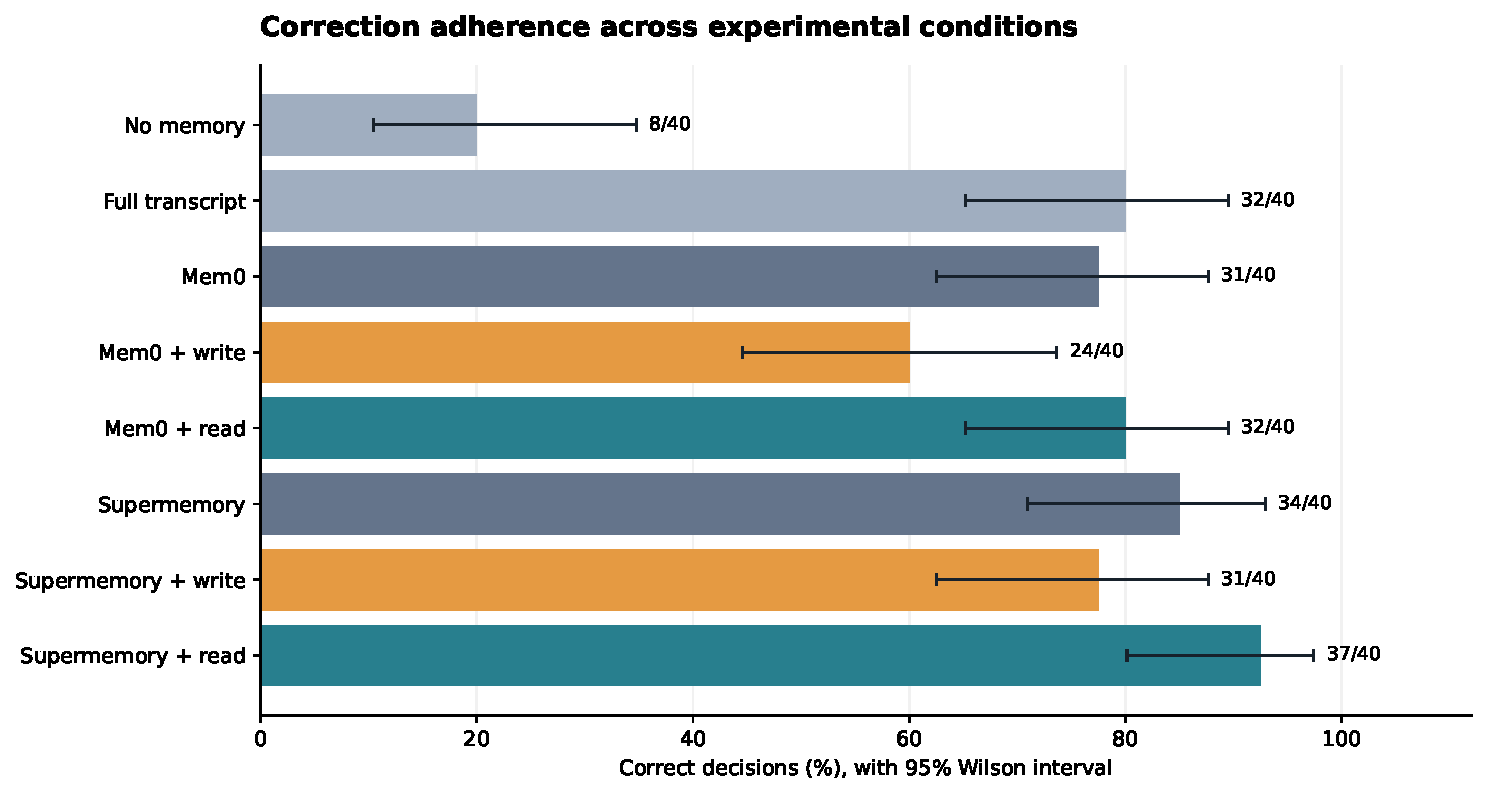
\includegraphics[width=0.86\linewidth]
    {01_overall_adherence.pdf}
\caption{Correction adherence across eight conditions
(40 episodes per condition); error bars are 95\% Wilson
intervals.}
\label{fig:overall-adherence}
\end{figure}

\subsection{Retrieval Versus Application}

Across the six memory-system conditions, 43 of 51
incorrect responses occurred despite retrieval of
the expected memory (Figure~\ref{fig:retrieval-gap}).
Unmodified Mem0 and Supermemory retrieved the
expected memory in all 40 episodes but made nine
and six incorrect decisions, respectively.
Read-time tagging reduced these counts to eight
and three.

Thus, successful retrieval is insufficient for
correct application, although a retrieved note
may still have lost important scope information.

The cleanest evidence comes from the full-transcript
control, where retrieval is perfect by construction yet
8 of 40 answers are wrong. All four single-task B probes
(\texttt{st-01b} to \texttt{st-04b}) fail even though each
probe states it is a new task, so the agent carried a
one-off exception into the next task. Retrieval is also an
easy step here: each pair has only 3.3 reference memories on
average (66 over 20 pairs) and ten results are returned, so
near-complete retrieval is expected.
Table~\ref{tab:retrieval-action} gives the full breakdown.

\begin{table}[htbp]
\centering
\small
\caption{Retrieved the expected memory vs acted correctly
(episodes out of 40). No memory counts as not retrieved;
the full transcript as retrieved.}
\label{tab:retrieval-action}
\begin{tabular}{lrrrr}
\toprule
Condition & Right/right & Right/wrong & Wrong/right & Wrong/wrong \\
\midrule
No memory & 0 & 0 & 8 & 32 \\
Full transcript & 32 & 8 & 0 & 0 \\
Mem0 & 31 & 9 & 0 & 0 \\
Mem0 + write & 23 & 9 & 1 & 7 \\
Mem0 + read & 32 & 8 & 0 & 0 \\
Supermemory & 34 & 6 & 0 & 0 \\
Supermemory + write & 31 & 8 & 0 & 1 \\
Supermemory + read & 37 & 3 & 0 & 0 \\
\bottomrule
\end{tabular}
\end{table}

Columns give retrieval/action (``right/wrong'' = retrieved right,
acted wrong).

\begin{figure}[htbp]
\centering
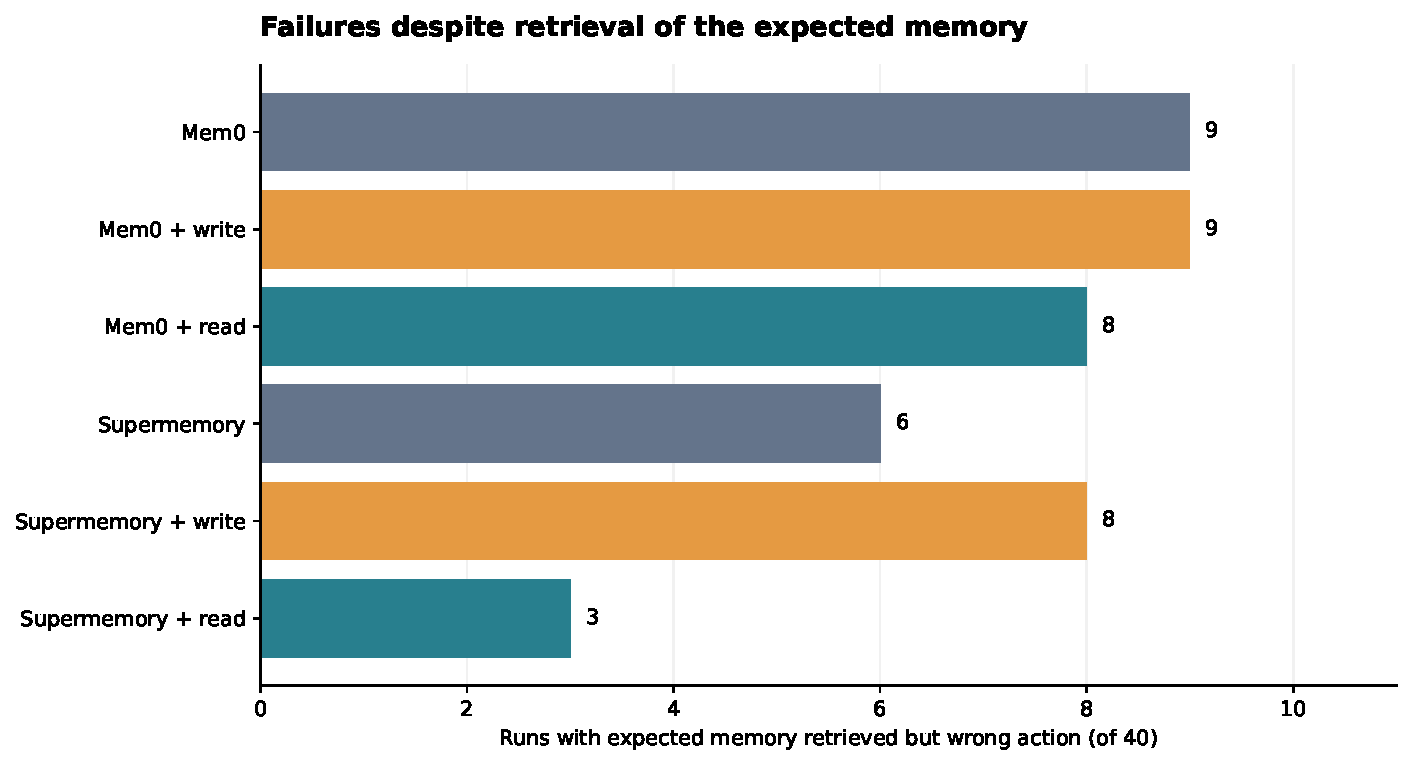
\includegraphics[width=0.82\linewidth]
    {02_retrieved_but_wrong.pdf}
\caption{Share of episodes with a wrong action when the
expected memory was retrieved (counts over the episodes where
it was retrieved). The full transcript counts as retrieved.}
\label{fig:retrieval-gap}
\end{figure}

\subsection{Scope-Boundary and Conflict-Type Performance}

Figure~\ref{fig:scope-boundaries} reveals asymmetric
write-time errors. Mem0 + write correctly handles
10/20 in-scope probes, versus 17/20 for Mem0.
Supermemory + write handles 11/20, versus 18/20
for its baseline, but correctly handles all 20
out-of-scope probes. This indicates substantial
under-application of scoped instructions.

Supermemory + read-time handles 20/20 in-scope
and 17/20 out-of-scope probes.

Table~\ref{tab:error-types} shows the direction of the
errors. The baselines lean toward over-application (Mem0 5
over-applied vs 4 under-applied; Supermemory 4 vs 1). Write-time tagging shifts
errors toward under-application (Mem0 9 vs 4; Supermemory
8 vs 0), and Supermemory + read-time makes no
under-application errors.

\begin{table}[htbp]
\centering
\small
\caption{Direction of wrong answers (episodes out of 40).
Over-applied: a memory outside its scope was used.
Under-applied: a broader or less specific memory was used.}
\label{tab:error-types}
\begin{tabular}{lrrrr}
\toprule
Condition & Over & Under & Superseded & Hedged/other \\
\midrule
Full transcript & 4 & 3 & 0 & 1 \\
Mem0 & 5 & 4 & 0 & 0 \\
Mem0 + write & 4 & 9 & 1 & 2 \\
Mem0 + read & 4 & 4 & 0 & 0 \\
Supermemory & 4 & 1 & 0 & 1 \\
Supermemory + write & 0 & 8 & 0 & 1 \\
Supermemory + read & 3 & 0 & 0 & 0 \\
\bottomrule
\end{tabular}
\end{table}

\begin{figure}[H]
\centering
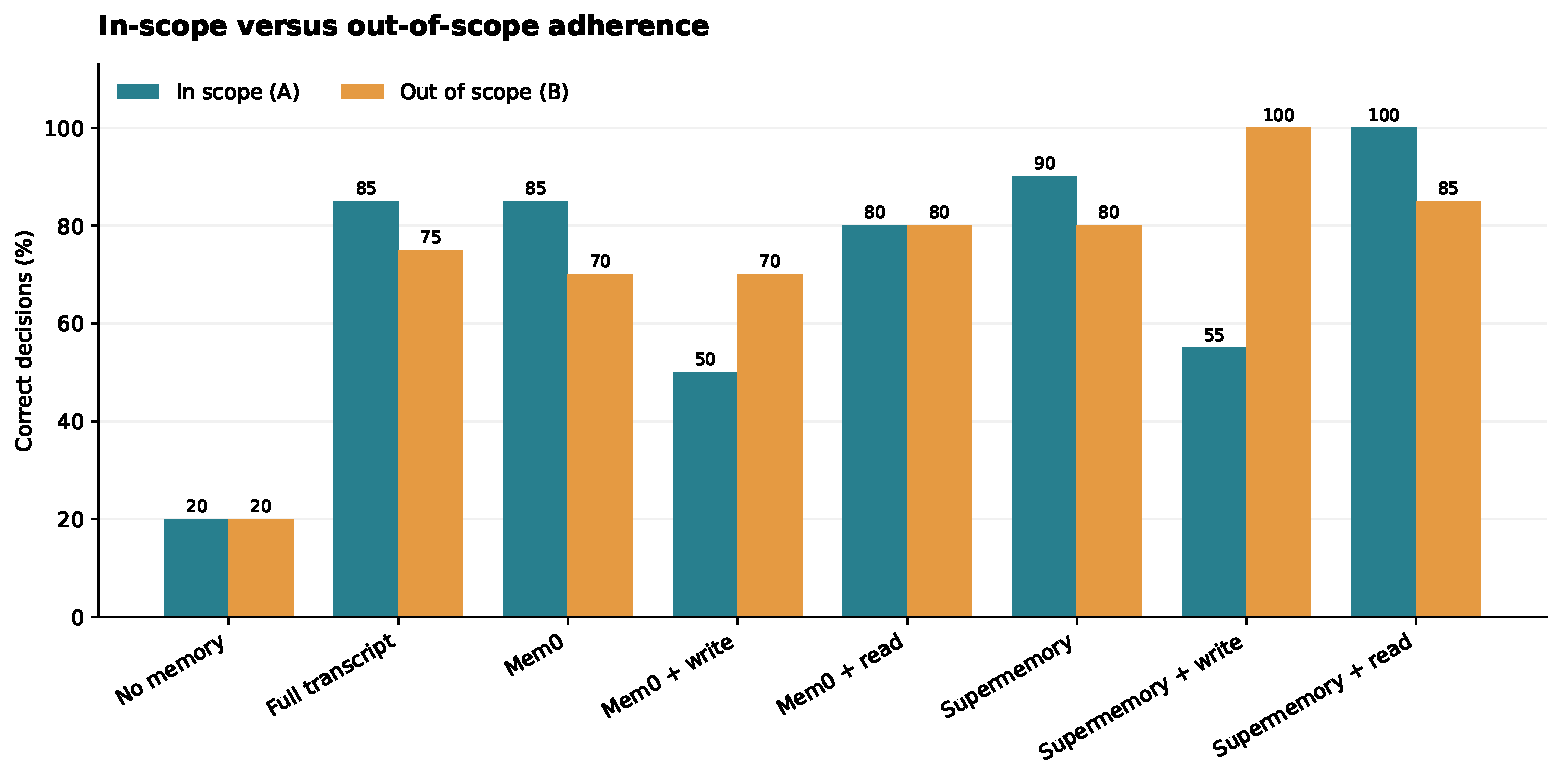
\includegraphics[width=0.86\linewidth]
    {03_in_scope_vs_out_scope.pdf}
\caption{Adherence on in-scope (A) and out-of-scope
(B) probes, 20 of each per condition.}
\label{fig:scope-boundaries}
\end{figure}

Across conflict types (Figure~\ref{fig:conflict-types}),
conditional scope and same-scope supersession are
handled reliably by most memory-system conditions.
Single-task overrides are hardest: Mem0 and
Supermemory each achieve 4/8, while read-time
Supermemory reaches 6/8. Same-scope specificity
also remains challenging, with 4--7/8 correct
among the full-transcript and memory conditions.

\begin{figure}[H]
\centering
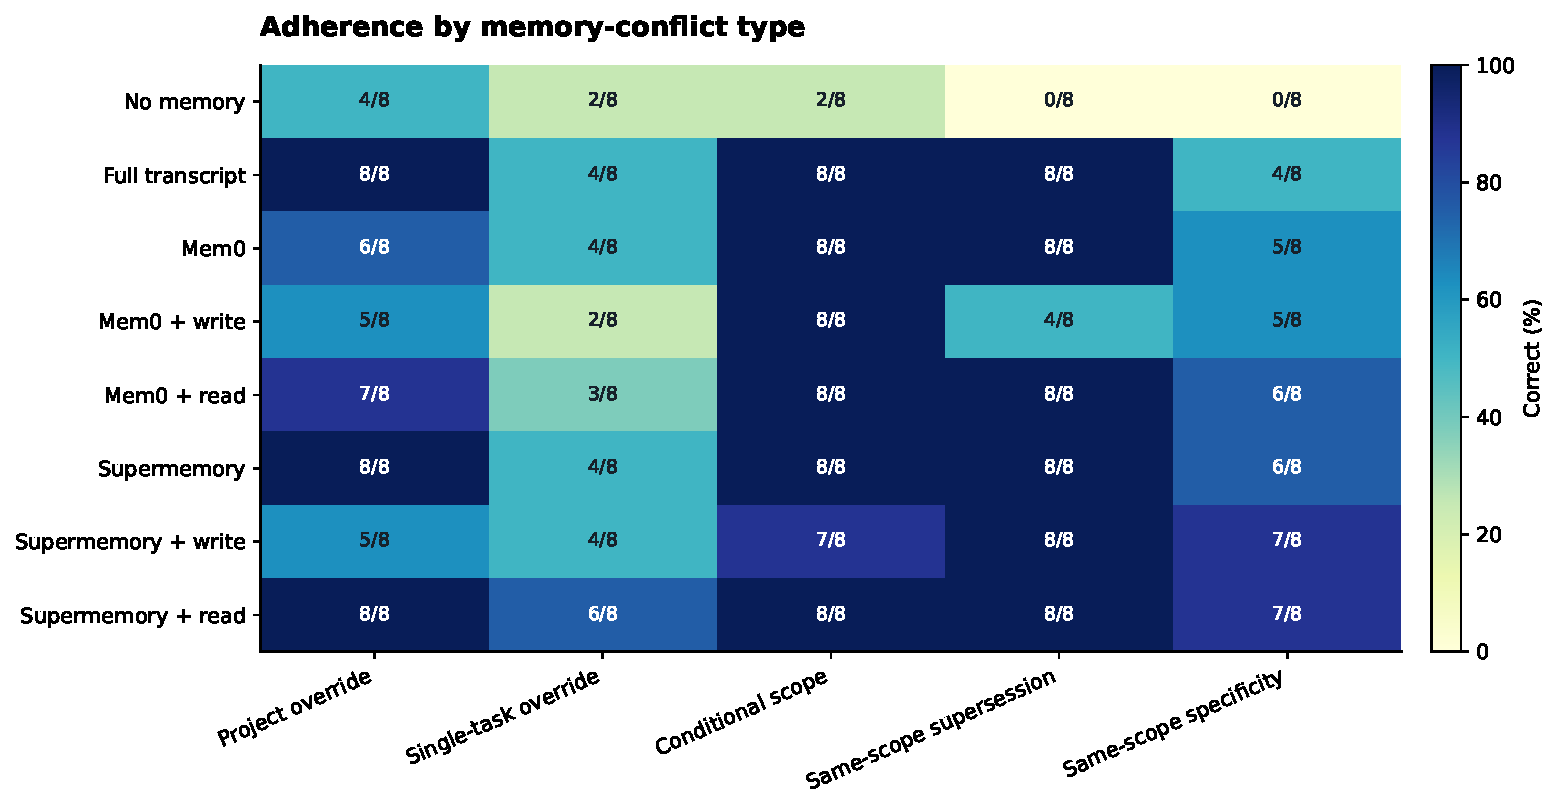
\includegraphics[width=0.88\linewidth]
    {04_conflict_heatmap.pdf}
\caption{Adherence across five conflict categories;
eight episodes per category.}
\label{fig:conflict-types}
\end{figure}

\subsection{Failure Diagnosis, Tagging, and Retention}

The diagnostic breakdown in
Figure~\ref{fig:failure-stages} attributes most
Supermemory baseline errors to reasoning despite
available information. Mem0 exhibits five baseline
scope-loss errors; write-time Mem0 has seven
extraction and four tagging failures among its
16 incorrect responses. Supermemory + write-time
has eight reasoning-classified failures among nine.

\begin{figure}[H]
\centering
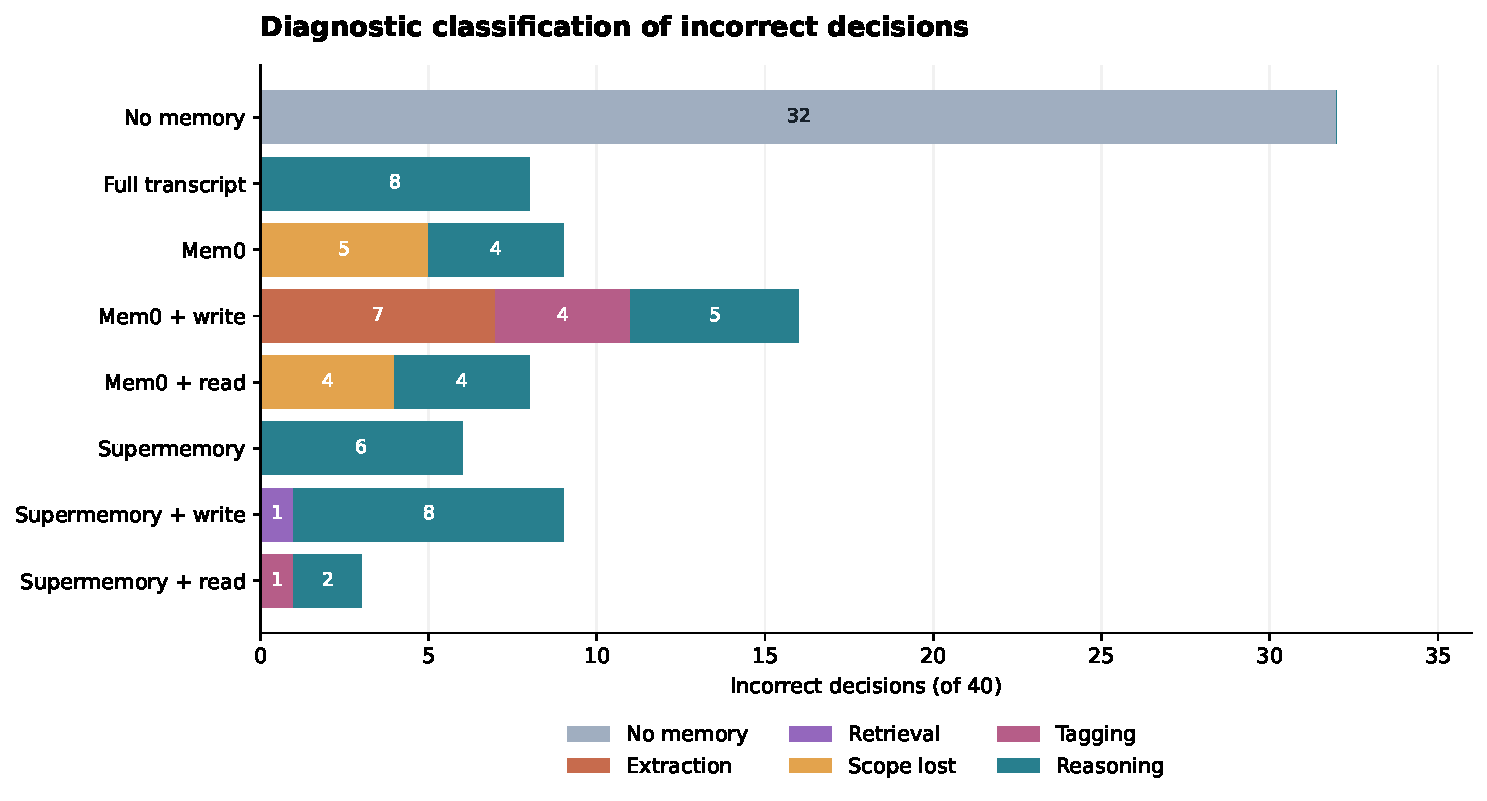
\includegraphics[width=0.84\linewidth]
    {05_failure_stages.pdf}
\caption{Incorrect decisions by earliest detected
failure stage; classifications are heuristic.}
\label{fig:failure-stages}
\end{figure}

Write-time tagging achieves 100\% scope accuracy
on evaluated tags for both systems (124 tags each),
versus 87\% for read-time Mem0 (111 tags) and 77\% for
read-time Supermemory (52 tags). For Mem0, only 97 of the 124
write-time tags came back after storage, consistent with
its re-extraction of the stored instructions. Read-time
Supermemory mislabels project memories as standing six
times, the commonest confusion there. Nevertheless, the highest downstream
adherence occurs with read-time Supermemory,
illustrating that tag accuracy alone is insufficient.
These figures use different eligible-note sets
and are not directly controlled comparisons.

Unrelated-memory retention is 95\% with the full
transcript, 67.5\% with Mem0, and 97.5\% with
Supermemory. Scope-aware Mem0 variants retain
62--72\%, compared with 87--98\% for
Supermemory variants. Mem0's retention is
significantly below the full transcript's
(1 episode vs 12, $p=0.003$), the largest paired
difference between a memory system and the control.
Scope tagging does not change retention significantly for
either system (all $p>0.2$). Read-time tagging held
retention level (Mem0 67\%$\to$72\%; Supermemory
98\%$\to$98\%), while write-time tagging
lowered it in both (Mem0 68\%$\to$62\%; Supermemory
97\%$\to$87\% on assessable episodes).

\begin{table}[htbp]
\centering
\small
\caption{Mean OpenRouter cost per episode. Supermemory's own
processing is billed separately and is not included.}
\label{tab:cost}
\begin{tabular}{lrr}
\toprule
Condition & USD / episode & Prompt tokens \\
\midrule
No memory & 0.00012 & 161 \\
Full transcript & 0.00013 & 465 \\
Mem0 & 0.00075 & 19,862 \\
Mem0 + write & 0.00102 & 33,799 \\
Mem0 + read & 0.00093 & 21,954 \\
Supermemory & 0.00012 & 444 \\
Supermemory + write & 0.00034 & 4,571 \\
Supermemory + read & 0.00024 & 2,597 \\
\bottomrule
\end{tabular}
\end{table}

Mem0's internal extraction calls make its baseline about 6
times as expensive per episode as the Supermemory baseline on
OpenRouter, and its scope-tagged variants 3--4 times as
expensive as their Supermemory counterparts. Supermemory's own
billing is excluded from this comparison.

\section{Discussion and Limitations}

\subsection{Write-Time versus Read-Time Tagging}

Read-time tagging matches or exceeds adherence
relative to both memory-system baselines, whereas
write-time tagging scored lower in both (not
significantly so against either baseline). For
Mem0 the logs point to a concrete cause: each
pre-extracted, pre-tagged instruction is passed
through Mem0's own extraction again, so 27 of 124
tags were lost (97 returned), 7 of 16 wrong answers
are classified as extraction failures, and prompt
tokens rise from about 19.9k to 33.8k per episode.
This is a property of our integration rather than
of write-time tagging itself; storing the tagged
instruction without re-extraction would test it.

For Supermemory no extraction loss is visible, and 8 of
its 9 wrong answers are classified as reasoning. One
possible explanation, which we did not test, is that
write-time extraction separates instructions from the
conversation that made their scope clear, making task
continuity harder to infer. Write-time Supermemory
illustrates the trade-off: it avoids over-applying
scoped memories on all 20 out-of-scope probes but
fails to apply many scoped instructions when
appropriate (8 under-applications).

Read-time tagging with Supermemory also works at a coarser
grain than Mem0's: Supermemory returns whole session
passages, so one tag describes everything in a passage, which
may help explain its lower tag accuracy (77\%). That coarseness
does not explain every error. In \texttt{sp-02b} the passage
was tagged with the correct condition (\texttt{recipient ==
neighbour}), yet the agent reasoned that a landlord counts as a
neighbour (Appendix~\ref{app:qualitative-failures}).

\subsection{Why Retrieval and Tagging Are Insufficient}

The retrieval--application gap shows that access
to a relevant instruction does not ensure correct
conflict resolution. In pair \texttt{po-01}, for
example, an agent may select the standing Polars
preference despite the applicable project-specific
pandas instruction. Other failures involve
carrying a single-task exception into a new task
(the full-transcript control does this on all four
single-task B probes) or combining conflicting
instructions.

These cases suggest that effective memory requires
both relevant information and reliable contextual
decision-making. Representative examples are
included in Appendix~\ref{app:failure-cases}.

\subsection{Threats to Validity}

The benchmark contains only 20 synthetic pairs
with short histories and explicit scope cues.
Nineteen pairs were initially AI-assisted, and
numeric conditions avoid threshold boundaries.
The findings may not generalize to longer,
ambiguous, or naturally occurring interactions.
Histories are short enough that retrieval is an easy
step (3.3 reference memories per pair against ten results
returned), so the retrieval--application gap is measured
under favourable retrieval conditions.

The study uses one agent model and one run per
condition. Fixed sampling settings do not
guarantee reproducibility, while Supermemory's
hosted processing is not fully observable.

The scope treatments jointly change metadata,
resolution instructions, and memory ordering,
preventing attribution of observed effects to
scope tags alone. Retrieval matching and
failure-stage diagnoses were not independently
validated in full. The gold labels were reviewed
against the drafts, but the committed annotation
files are identical, so no independent
inter-annotator agreement is available.

The vendor claim check planned in the project
design (a LongMemEval subset run through
MemoryBench) was not carried out, so this report
makes no comparison with vendors' published
figures.

Finally, the two probes within each pair are
dependent, limiting the interpretation of
episode-level significance tests.

\section{Conclusion}

We evaluated whether scope-aware memory handling
helps agents apply retrieved instructions in
the correct context. Across 320 runs, incorrect
memory application frequently occurred even when
the expected memory was retrieved.

Read-time tagging with Supermemory achieved the
highest observed adherence (not significantly above
its baseline), while write-time tagging scored lower
for both memory systems. Read-time tagging did not
lower unrelated-memory retention; write-time tagging
did lower it, though not significantly. The results
suggest that scope-aware interventions may be useful,
but explicit metadata alone does not resolve
contextual memory conflicts. Larger benchmarks and
controlled ablations are needed to isolate
the effects of tagging, conflict-resolution
instructions, and memory ordering.

\section*{Individual Contributions}

% Replace with verified contributions and shares
% summing to 100 percent.
\begin{table}[htbp]
\centering
\small
\begin{tabularx}{\linewidth}{lXr}
\toprule
Member & Contributions & Share \\
\midrule
Isaac Chin Wei En & Environment and baseline integration; episode schema, scope-labelling guide and 20-pair benchmark; automated validation and leakage checks; agent-model selection pilot & -- \\
Edward Chew Kian Boon & Scope layer and logging & -- \\
Ng Cheng Kiat Nicholas & Evaluation and scoring & -- \\
Jagan Mohan Shailesh & Validation, analysis, report & -- \\
\bottomrule
\end{tabularx}
\end{table}

\bibliographystyle{plainnat}
\bibliography{references}

\appendix


\section{Episode Examples and Qualitative Failure Analysis}
\label{app:failure-cases}

\subsection{Episode JSON Structure}
\label{app:episode-schema}

Each benchmark pair is stored as a JSON file under
\path{episodes/pairs/}. The file contains the shared
conversation history, reference memories, two evaluation
probes, and an unrelated-memory retention check.
Table~\ref{tab:episode-schema} summarises the top-level
fields.

\begin{table}[htbp]
\centering
\small
\caption{Top-level fields of an episode-pair JSON file.}
\label{tab:episode-schema}
\begin{tabularx}{\linewidth}{lX}
\toprule
Field & Description \\
\midrule
\texttt{pair\_id} &
Unique identifier of the paired scenario. \\

\texttt{conflict\_type} &
Type of memory conflict being evaluated. \\

\texttt{domain} &
Specific decision domain, such as dataframe library. \\

\texttt{domain\_kind} &
Broader category of the task domain. \\

\texttt{sessions} &
Ordered earlier conversations containing user
instructions and contextual information. \\

\texttt{memories} &
Reference instructions extracted from the sessions,
including their source, role, intended action,
and gold scope annotations. \\

\texttt{probes} &
Two evaluation tasks (A and B) sharing the same
history but differing in contextual applicability.
Each specifies its expected action and winning memory. \\

\texttt{retention\_checks} &
Requirements testing whether unrelated standing
preferences are preserved. \\
\bottomrule
\end{tabularx}
\end{table}

Each session contains a \texttt{session\_id},
chronological \texttt{order}, \texttt{task\_id},
\texttt{active\_project}, and conversation
\texttt{text}.

Each reference memory contains a \texttt{memory\_id},
source \texttt{session\_id}, instruction \texttt{text},
\texttt{role}, \texttt{decision}, \texttt{action},
and a \texttt{gold} object. The latter specifies
\texttt{scope}, \texttt{key}, and \texttt{condition}.

Each probe contains a task identifier, project context,
natural-language request, structured \texttt{facts},
an \texttt{in\_scope} indicator, the decision being
tested, \texttt{expected\_action},
\texttt{expected\_memory}, and \texttt{deciding\_rule}.

The \texttt{retention\_checks} array identifies
an unrelated memory and the requirement used
to evaluate whether it is followed.

Only the conversation sessions and the selected
probe text are supplied as episode inputs to
the experimental systems. Reference memories,
structured context, gold labels, and expected
outcomes are reserved for validation and scoring.

\subsection{Complete Example: Project Override
(\texttt{po-01})}
\label{app:po01-example}

Pair \texttt{po-01} illustrates the mirrored-pair
design. Two earlier sessions establish three
reference memories: a standing preference for
Polars on datasets exceeding one million rows,
a project-specific instruction to use pandas
for Project Marlin, and an unrelated requirement
for Python type hints.

Probe A concerns Project Marlin, where the
project-specific instruction takes precedence.
Probe B changes only the project to Project Tern,
where the standing Polars preference applies.
Both probes independently test retention of
the type-hint instruction.

Listing~\ref{lst:po01} reproduces the complete
JSON specification used by the benchmark.

\lstinputlisting[
    style=jsonstyle,
    caption={Complete JSON specification of
    project-override pair \texttt{po-01}.},
    label={lst:po01}
]{../episodes/pairs/po-01.json}

\subsection{Qualitative Failure Cases}
\label{app:qualitative-failures}

The following cases illustrate distinct
memory-application failures observed in the
experimental evaluation.

\subsubsection{Project Override:
\texttt{po-01}}

The user generally prefers Polars for datasets
exceeding one million rows but requires pandas
for Project Marlin.

Probe A concerns Marlin and expects pandas,
whereas Probe B concerns Project Tern and
expects Polars. The unrelated type-hint
preference applies to both.

On Probe A, four conditions chose Polars where
pandas was expected: Mem0, both scope-tagged Mem0
variants, and write-time scope-tagged Supermemory.
In all four, the Marlin pandas instruction was among
the retrieved memories, and the failure was in the
agent's reasoning. Plain Mem0 opened its answer with
``Use Polars for this 5M-row dataset to ensure high
performance and memory efficiency.'' In both tagged
Mem0 variants, the tagger had labelled the Marlin
memory as project scope with key Project Marlin and
the Polars memory as standing scope, yet the agent
still applied the standing rule.

The full-transcript, Supermemory and read-time
scope-tagged Supermemory conditions chose pandas on
Probe A. All seven conditions with memory chose Polars
on Probe B, as expected. Retrieving the applicable
instruction therefore did not ensure that the agent
applied it over a conflicting standing preference.

\subsubsection{Single-Task Override:
\texttt{st-01}}

The user usually exports tables as parquet, but for
one client-churn export asks for CSV because the
retention team opens it in Excel.

Probe A continues that job and expects CSV. Probe B
begins ``New task, client churn export job: \ldots''
and expects the standing parquet preference.

On Probe B the full-transcript control, read-time Mem0
and read-time Supermemory all answered with CSV; in
read-time Mem0 the note recording the CSV request reached the
agent untagged, and the agent opened with ``Format: CSV.''
The same pattern appears on all four single-task pairs in the
full-transcript control, so the failure is in the agent's
handling of task continuity, not in what was retrieved.

\subsubsection{Same-Scope Specificity:
\texttt{sp-02}}

The user normally begins emails with
``To whom it may concern,'' but when writing to a
neighbour wants ``Hey there,''.

Probe A asks for an email to a neighbour and
expects the conditional greeting. Probe B asks for
an email to a landlord and expects the default.

On Probe A, plain Supermemory produced both greetings
(``Hey there, To whom it may concern,''), which the judge
labelled mixed. On Probe B, read-time Supermemory returned a
passage tagged with the correct condition
(\texttt{recipient == neighbour}), yet the agent wrote that it
``applied the neighbour-specific opening rule \ldots\ as the landlord
is a person in the user's building.'' The failure-stage
classifier labelled this case a tagging error; on the
evidence above it is better described as the agent stretching
the condition.

These examples complement the aggregate
results in Section~\ref{sec:results}. The retrieved notes,
responses and judge labels for a representative sample are
in \texttt{reports/examples.md}; the full per-run logs are
not committed (Appendix~\ref{app:reproducibility}).

\subsection{Agent Prompt and a Rendered Example}
\label{app:prompt}

The same prompt template is used in every condition; only
the \texttt{\{memories\}} text changes.

\begin{lstlisting}[basicstyle=\ttfamily\scriptsize,breaklines=true,frame=single]
You are an assistant helping a user with data and software
work. Below are memories saved from the user's earlier
conversations, followed by their current request. Use the
memories that apply to this request and ignore the ones that
do not.

Memories:
{memories}

Current request:
{probe}

Respond with your answer. State the concrete choice you made
(for example the tool, format or approach) in the first line.
\end{lstlisting}

For \texttt{po-01a} under read-time Mem0, the memories slot
held six retrieved notes, for example ``User is starting
Project Marlin \ldots\ and has mandated the use of pandas''
tagged \emph{project, key: Project Marlin}, and ``User prefers
using the Polars library \ldots\ larger than 1 million rows''
tagged \emph{standing, condition: rows $>$ 1000000}, followed by
the resolution rules of Section~\ref{sec:scope-representation}.
The agent still answered ``I chose Polars \ldots\ triggering the
standing preference \ldots''


\section{Supplementary Experimental Results}
\label{app:supplementary-results}

The full pair-by-pair adherence matrix,
tagging-accuracy breakdown, failure-stage
counts, and per-condition cost accounting
are available in \path{reports/summary.md}
and \path{reports/episode_scores.csv}.

OpenRouter spending for the full experiment
was approximately \$0.15, with approximately
\$0.06 for judging. Supermemory's separately
billed processing is excluded.

\section{Reproducibility and Implementation Details}
\label{app:reproducibility}

The implementation is available in the project
repository. Experimental conditions are defined
in \texttt{agent/conditions.py}; runs are executed
through \texttt{agent/runner.py}; and scoring is
implemented in \texttt{scoring/}.

The per-run logs (\texttt{runs/logs/}) and the judge cache
are gitignored and are not in the repository; they were
produced on one team member's machine. The committed
\texttt{reports/} directory holds the scored outputs
(\texttt{episode\_scores.csv}, \texttt{tables/},
\texttt{examples.md}), so the tables and figures here can
be checked from the repository, but re-scoring from raw
logs needs those local files. Figures are generated from the
tables in \texttt{reports/tables/}.

\end{document}

